\documentclass[../main.tex]{subfiles}
\graphicspath{{\subfix{../images/}}}
\begin{document}

\label{Ex:EFT}\index{exercise!EFT}\index{exercise!affirmations}

\begin{figure}[htb]
  \centering
 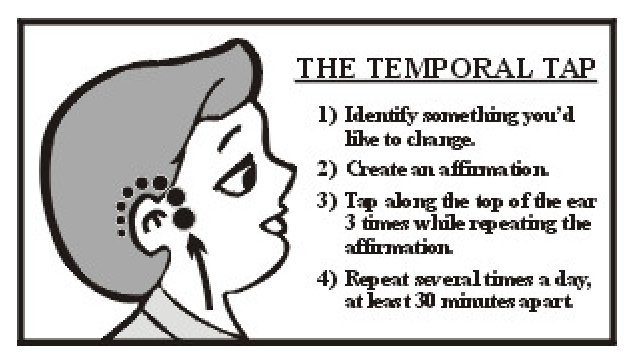
\includegraphics[width=6cm]{temptap.eps}      
\caption{Emotional Freedom Technique EFT}
\end{figure}

\mytextbox[0]{Gwenn Bonell pusblished the following article under the title "Transfrom your life with the temporal tap"~\cite{EFT}:
  \vspace{5mm}
   
  \noindent 
I was skeptical when I first heard about the Temporal Tap from Dr. Larry Nims.
Then I saw Donna Eden endorse it, and I began to think maybe there was something to this technique.
I began experimenting using the Temporal Tap with an affirmation\index{affirmation} to increase self-esteem and attract abundance.
Five days later, I was handed a totally unexpected check for over \$18,000! Within two weeks, our investments went up over \$75,000 AND we bought a house on the beach.
I was sold on the power of the Temporal Tap!

This energy technique helps break old habits\index{symptom!habits, old}, attitudes\index{symptom!attitudes, old}
or emotional responses\index{symptom!emotional responses} and establishing new ones.\index{effect!changing!habits} \index{effect!changing!pattern} \index{effect!changing!belief} 
Simply tapping on the head around the top of the ear calms the part of the nervous system that fights to maintain
your current belief systems\index{belief system} and patterns of behavior.\index{behavior!pattern}
The brain is then more receptive to learning new beliefs and instilling new affirmations.

Begin by identifying a habit\index{habit}, attitude\index{attitude}, or condition in your life\index{life!conditions} that you would like to change.
Then describe the change in a single sentence, and state it as an affirmation in present time as if the condition already exists.
For example, you could say, "I always have more than enough money to pay my bills," or "Right now, I am prosperous."
Affirmations can be anything you wish to become true and operative in your life.
They can be specific or general, and in your own language, your own lingo, and aligned with your own values.
For easy recall, make them short and to the point.


To perform the Temporal Tap, start tapping at your right temple in front of the ear canal and continue tapping on the scalp around the top edge of the ear
until you reach the back center of the ear, just opposite where you started.
The active spots are only along the upper half of the ear, from front center to back center.
Tapping with all your fingertips bunched together ensures that all the points along the Temporal--Sphenoidal (T--S) line are stimulated.
Say your affirmation while you tap; repeat this procedure three times.

Do this several times a day, waiting at least 30 minutes before repeating the same affirmation.
You can tap for as many different affirmations as you wish as long as you can easily address them all several times a day.
Reinforcement is part of the process. Once your affirmation has become a part of your life, you can replace it with a new one.

Temporal Tapping has helped people build confidence, optimism, and self-esteem while replacing old habits with constructive behavior.
It can be used for almost any area of your personal life, including mental, emotional, physical, spiritual, occupational, domestic, and social.
People have used it to lose weight, to improve job performance, and even to stop fingernail biting.
It is a simple yet powerful way to change many patterns or habits.
Focus on what part of your life you most want to change, and create a simple affirmation that reflects your highest ideals.
}

\mytextbox[0]{
  Perceive exactly, what goes through your head when you speak your affirmation out loud.
If you say for phrase it ``I deserve wealth and oppulence in life'' and your inner voice answers
``That's no good, I'm not sufficiently educated (raised) to be rich", that means your affirmation isn't right for you and has to be adapted.

Instead, you could maybe say: ``I'm now in the position to recognize chances which creat wealth and to use them''; this could be more effective.
So when you phrase it ``Money easily flows into my life'' and the following words come up: ``My parent lived from bill to bill and that's exactly how I want it to be'',
maybe you can try ``I'm wealthier than my parents, because they choose to live that way''.

Be creative with your affirmations and find the ones which fit for you and in which you truly can believe.
For instance, affirmations can sound like ``I constantly do everythin necessary to sustainably change my life towards a positive stream of income'',
``The universe is always helping me'' or ``Everything I touch will be a success''.

One of my students used the phrase ``My income grows, regardless if I work, sleep or play'' and got the next that he applied for.
Other students had in their affirmations the element ``I help a lot of people'' and ``I make tons of money''.
Soon after, they used their chances to increase the customer base and their income.
Now they are using the affirmation ``I make at least \$500 a week".

  }
\end{document}